\documentclass{sig-alternate-05-2015}
\usepackage{cite}
\usepackage{amsmath}
\usepackage{tcolorbox}
\usepackage{pdfpages}
\usepackage{hyperref}
\usepackage{booktabs}

\newcounter{qcounter}


\begin{document}

% Copyright
\setcopyright{acmcopyright}

% DOI
\doi{10.475/123_4}

% ISBN
\isbn{123-4567-24-567/08/06}

%Conference
\conferenceinfo{EMSE '16}{March 28--June 10, 2016, Corvallis, OR, USA}

\acmPrice{\$15.00}

\title{Conflicts of Interest: Merge Conflict Resolution Patterns in Open Source Projects}
\subtitle{Empiricial Methods of Software Engineering (EMSE), Spring 2016}

\numberofauthors{2}

\author{
\alignauthor
	Shane McKee\\
       	\affaddr{Oregon State University}\\
       	\affaddr{2500 NW Monroe Avenue}\\
       	\affaddr{Corvallis, Oregon}\\
       	\email{mckeesh@oregonstate.edu}
\and
\alignauthor
Nicholas Nelson\\
       \affaddr{Oregon State University}\\
       \affaddr{2500 NW Monroe Avenue}\\
       \affaddr{Corvallis, Oregon}\\
       \email{nelsonni@oregonstate.edu}
}


\maketitle
\section{Introduction}\label{Introduction}
Collaboration between software developers working on the same project carries the risk of discord and incongruity. Within software projects that use Distributed Version Control Systems (DVCS), these issues can appear in the form of merge conflicts. With 28.4\% of all projects on Github being non-personal repositories (as of Jan. 2014), the prevalence of merge conflicts is significant \cite{kalliamvakou14}. Since merge conflicts carry a cost to any software project, developers and researchers have pursued ways of mitigating them \cite{niu2012}. But mitigation strategies must be based upon a foundation of understanding both the problem space --- conflicting versions of code --- and the factoring that contribute to their occurrence.

Popular version control systems (i.e. \texttt{Git}, \texttt{SVN}, \texttt{Mercurial}, \texttt{Bazaar}) have features that allow for the detection of merge conflicts, and can automatically resolve a subset of these conflicts using basic merging strategies. For example, \texttt{git} (the current VCS leader with 29\% of developers selecting it as their primary VCS according to a 2013 study by Ohloh~\cite{German16}), provides the following merge strategies: \textit{resolve}, \textit{recursive}, \textit{rebase}, \textit{octopus}, \textit{ours}, and \textit{subtree}. But when more complex conflicts occur, these version control systems require developer intervention to resolve the conflict. Although several papers have examined how and why merge conflicts occur \cite{brun10}\cite{Sarma08}\cite{Guimaraes12}, little attention has been paid to understanding how developers resolve merge conflicts in practice.

By mining software repositories on Github for instances of merge conflicts, and examining the resolution patterns that developers took to resolve them, we are able to highlight both the current strengths and the potential deficiencies within current version control systems. Our results show that certain resolution patterns are more prevalent within the broader open-source community, and that tool developers should focus on these particular patterns when evolving and adding to the automated systems and algorithms available for software development and project collaboration.

\begin{table*}
\centering
\caption{Executive Summary}
\begin{tabular}{| l | p{10cm} | } \hline
Goal & To understand merge conflict resolution patterns in Git repositories. \\ \hline
Research Questions  & \textbf{RQ1:} What merge conflict resolution patterns exist in Git?\\
& \textbf{RQ2:} What is the frequency distribution of merge conflict resolution patterns by programming language?\\
& \textbf{RQ3:} Is there a relationship between the size of the conflict and its conflict resolution pattern?\\ \hline
Empirical Method & This project used data mining. Data mining was best for RQ1 because it gave us the least biased view of what developers do to resolve conflicts in practice. It was best for RQ2 because it allowed us to get a sample across a wide variety of languages while testing for certain resolution patterns. It was best for RQ3 because it was easy to extract the size of a conflicted area and compare it to the type of merge conflict resolution that was used.\\ \hline
Data Collected & Number of merges, number of merge conflicts, size of each conflict, pattern used in each resolution, primary programming language of each project.\\
\hline\end{tabular}
\label{table:t1}
\end{table*}

\section{Background}\label{Background}

Modern version control systems base their representations of code, and the underlying changes upon it, on graph theory. These models provide an entire family of models and methods for evaluating and attempting to resolve merge conflicts, but are limited either by the bounds of a particular model or the accuracy of its heuristics \cite{ehrig15} \cite{mens99}. We base our assumption that certain merge conflicts cannot be resolved by version control systems, and thus require human intervention, on these fundamental limitations in graph modeling.

Merge algorithms are an area of active research, and consequently there are many different approaches to automatic merging, with subtle differences. The more notable merge algorithms include three-way merge \cite{livshits07}, recursive three-way merge, fuzzy patch application \cite{brunet06}, weave merge \cite{nguyen07}, and patch commutation. These concepts form both a model of understanding and a lens for us to examine the differences between the theoretical models and real-world application.

Our research is guided by prior work into conflict detection and automated conflict resolution. Brun, et al. \cite{brun11}, ML Guim\~{a}raes, et al. \cite{Guimaraes12}, C Schneider, et al. \cite{schneider04}, and Dewan et al. \cite{dewan07} have all attempted to locate current and upcoming merge conflicts as early as possible in order to prevent them from occurring. We take the approach that some conflicts cannot be detected either by collaborator awareness or by proactively engaging automated merging tools, and that understanding how developers currently adapt to such situations is fundamental to developing tools that support such situations.\\

\section{Study Design}\label{design}
\subsection{Aspects of software development considered} 
\subsubsection{Motivations}
Merge conflicts have become a popular area of study, perhaps due to the importance of version control in the developer workflow or developers' dislike for resolving messy merge conflicts. Resolving a merge conflict can require extra time to understand how the two sets of new code should be integrated together. Therefore, we focus our attention on the patterns that developers engage in when actively resolving such merge conflicts. Our results will hopefully provide both impetus and emphasis for further VCS development and the creation of tools that target specific resolution patterns.
\subsection{Dataset}
Our data was selected from the most popular open-source projects on GitHub. We used the star ratings assigned to projects hosted on GitHub as a metric for the popularity of the project, selecting only projects that were ranked within the top 30 projects according to this metric (as of May 2016). We further filtered our selections to remove projects such as \textit{legacy-homebrew}, \textit{gitignore}, \textit{html5-boilerplate}, \textit{You-Dont-Know-JS}, \textit{Font-Awesome}, \textit{free-programming-books}. These projects either did not contain code in known programming languages (font templates, books, etc.) or were not collaborative projects likely to contain merge conflicts (collections of scripts, sample programs, etc.). We thus excluded them from our corpus.

Within. The following data was gathered:
\begin{enumerate}
\item \textbf{Number of merges}\\
	This is the total number of merges, both automatically and manually merged. The intent is to identify what percentage the merges in our corpus must be manually merged.
\item \textbf{Number of merge conflicts}\\
	This is the number of merge conflicts that can be found using Git and GitPython. This will limit us to textual merge conflicts, but maintain or alignment with analyzing the patterns associated with resolving conflicts that occur when merging within an open source project.
\item \textbf{Size of each conflict}\\
	We will determine the size of a conflict between commit A and commit B by the following equation:\\ 
	$$\text{SLOC}(\text{git diff}(Original, A))$$
	$$+$$
	$$\text{SLOC}(\text{git diff}(Original, B))$$
\item \textbf{Pattern used to resolve each conflict}\\
	Each merge conflict resolution was classified as one of the following patterns:
	\begin{enumerate}
	\item\textit{Take One:} Changes from one parent commit are taken while changes from the other parent commit are discarded.
	\item\textit{Interweaving:} Changes are taken from both commits in relatively equal portions and interweaved together in the resulting merge.
	\item\textit{Decline:} No changes are taken from either parent commit, and no new lines are added while resolving the merge conflict.
	\item\textit{Overwrite:} No changes are taken from either parent commit, and code is added while resolving the merge conflict.
	\item\textit{Other:} No pattern was found that conformed to the previously outlined patterns. 
	\end{enumerate}
\item \textbf{Primary programming language of each project}\\
Primary language is determined based upon the internal analysis of GitHub, which determines programming language on a per-file basis through the use of static syntax analysis and file extensions. Each project is designated with a programming language that is most prevalent in the files that are included within it.
\end{enumerate}

\begin{table*}
\centering
\caption{Corpus Description}
\begin{tabular}{| l | c | c | c | c | c | c | c | c | } \hline
\toprule
\textbf{Project} & \textbf{Language} & \textbf{Stars} & \textbf{Commits} & \textbf{Merges} & \textbf{Conflicts} \\ \hline
angular/angular.js & JavaScript & 49,777 & 7,839 & 137 & 14 \\ \hline
danedan/animate.css & CSS & 32,732 & 1,216 & 92 & 8 \\ \hline
robbyrussell/on-my-zsh & Shell & 38,097 & 3,977 & 1,468 & 35 \\ \hline
FreeCodeCamp/FreeCodeCamp & JavaScript & 136,24S & 8,548 & 333 & 22 \\ \hline
impress/impress.js & JavaScript & 27,550 & 261 & 114 & 17 \\ \hline
docker/docker & Go & 31,893 & 19,605 & 187 & 11 \\ \hline
rails/rails & Ruby & 31,471 & 34,599 & 2,371 & 121 \\ \hline
hakimel/reveal.js & JavaScript & 28,549 & 1,796 & 217 & 13 \\ \hline
nwjs/nw.js & JavaScript & 28,567 & 2,547 & 495 & 26 \\ \hline
d3/d3 & JavaScript & 63,206 & 3,716 & 68 & 4 \\ \hline
\bottomrule
\multicolumn{4}{l}{\footnotesize * Collected from GitHub on May 31-June 07, 2016}\\
\end{tabular}
\label{table:t2}
\end{table*}

\begin{table*}
\centering
\caption{Resolution Patterns}
\begin{tabular}{| l | c | c | c | c | c | c | c | c | } \hline
\toprule
& & \multicolumn{4}{c}{\textbf{Resolution Pattern Usage}} \\
\textbf{Project} & \textbf{Language} & \textit{TakeOne} & \textit{Interweaving} & \textit{Decline} & \textit{Overwrite} \\ \hline
angular/angular.js & JavaScript & 0 & 0 & 0 & 0 \\ \hline
danedan/animate.css & CSS & 0 & 0 & 0 & 0 \\ \hline
robbyrussell/on-my-zsh & Shell & 0 & 0 & 0 & 0 \\ \hline
FreeCodeCamp/FreeCodeCamp & JavaScript & 0 & 0 & 0 & 0 \\ \hline
impress/impress.js & JavaScript & 0 & 0 & 0 & 0 \\ \hline
docker/docker & Go & 0 & 0 & 0 & 0 \\ \hline
rails/rails & Ruby & 0 & 0 & 0 & 0 \\ \hline
hakimel/reveal.js & JavaScript & 0 & 0 & 0 & 0 \\ \hline
nwjs/nw.js & JavaScript & 0 & 0 & 0 & 0 \\ \hline
d3/d3 & JavaScript & 0 & 0 & 0 & 0 \\ \hline
\end{tabular}
\label{table:t3}
\end{table*}

\subsection{Data Gathering and Analysis}
Our dataset is comprised of project metadata, \texttt{git} logs, and commits gathered from GitHub through a combination of GitPython, GitHub API v3, and Python libraries. Our dataset was pulled from GitHub and analyzed locally in order to avoid exceeding the access limitations placed upon developers accessing GitHub data through the use of their APIs. We gathered this dataset using the following steps:\\
\begin{enumerate}
\item Clone local copies of the \texttt{master} branch version of top projects based upon number of stars, with the limitation that some projects were not suited for this type of research and were therefore excluded.
\item Collect all merges within the \texttt{master} branch of a repository.
\item Locate merge conflicts by speculatively merging two commits, and their accompanying branch histories.
\item Obtain the conflicting versions of each text section (\texttt{section A} from commit \texttt{A}, and \texttt{section B} from commit \texttt{B}) by parsing the unmerged sections resulting from the speculative merge.
\item Obtain the merge conflict resolution text section (commit \texttt{M}) by branching from parent \texttt{A}, merging parent \texttt{B} into that newly created branch, committing the resulting merge conflict as if it were resolved, taking the \texttt{diff} of the commit \texttt{M} and the merge conflict resolution.
\item Analyze \texttt{section A}, \texttt{section B}, and \texttt{section M} for each merge conflict resolution in order to categorize the resolution into one of the previously indicated classifications.
\end{enumerate}

\begin{figure*}[t]
\caption{Miner Architecture}
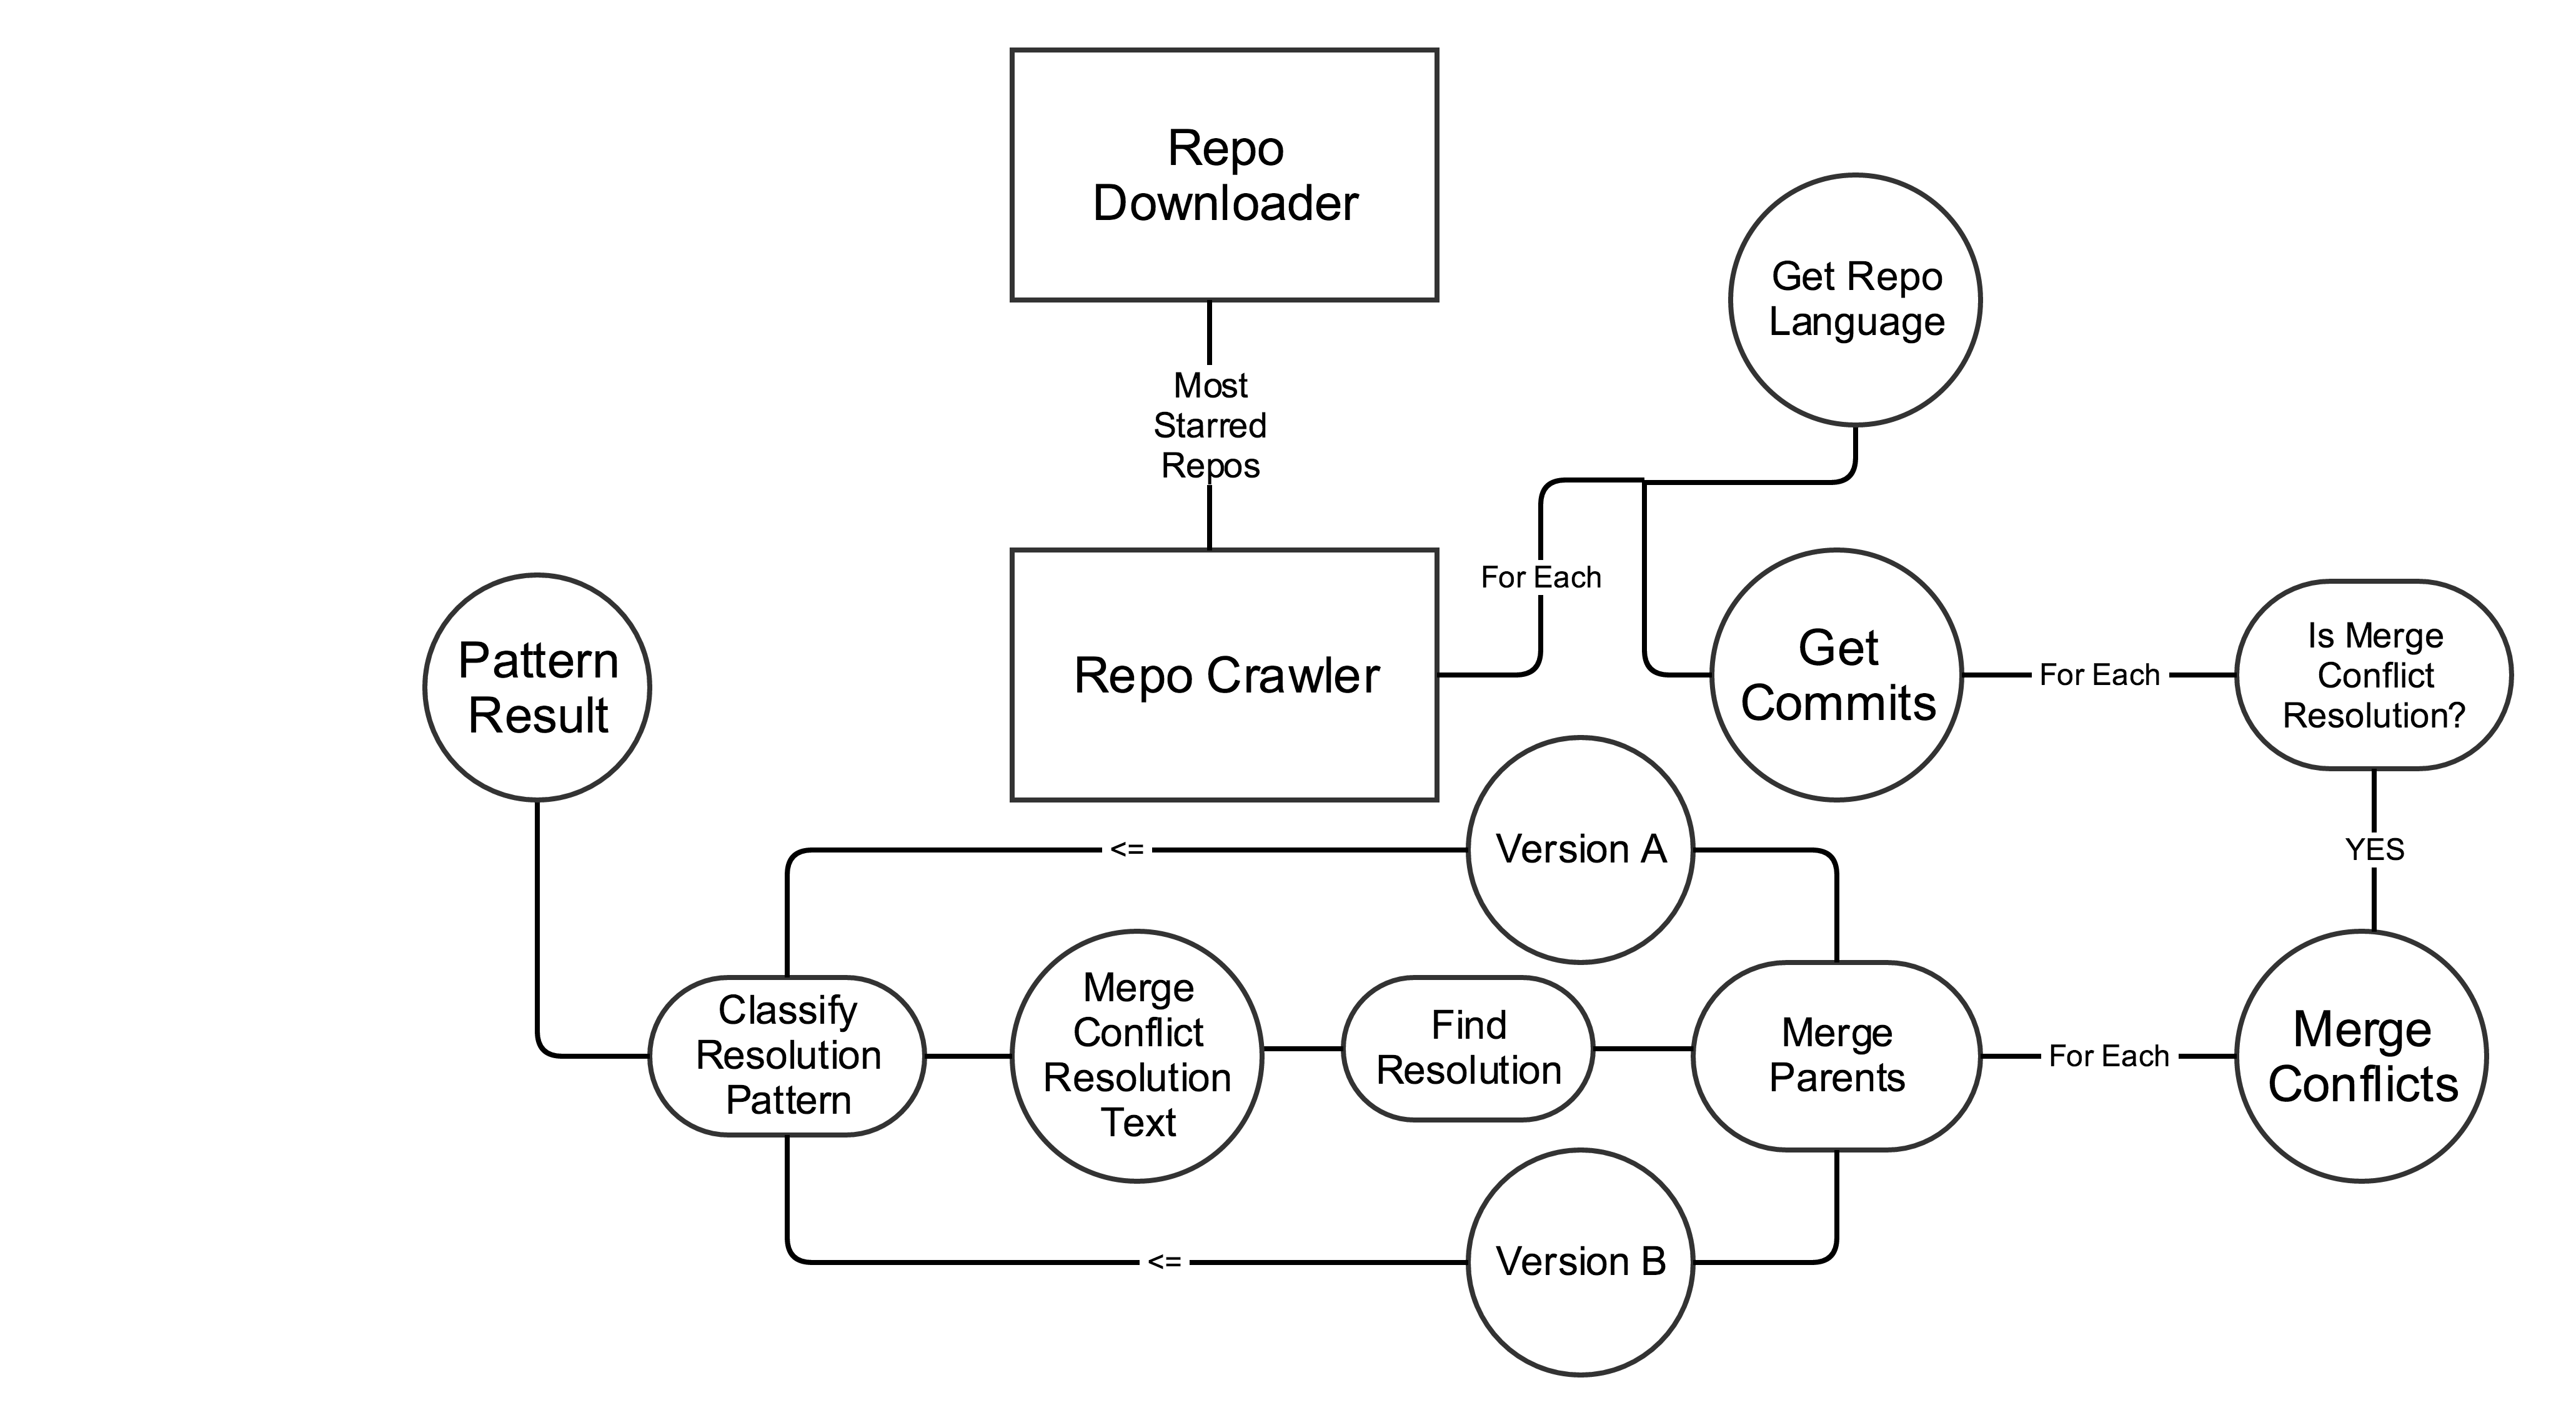
\includegraphics[width=\textwidth]{miningarchitecture}
\centering
\label{figure:f1}
\end{figure*}

Since most of the repositories not suitable for this research were already removed prior to this analysis process, the resulting dataset required only minimal manual pruning prior to conducting population analysis. 

Our study will be limited by both space and time. Since we must store the project metadata and each target commit while mining a Github repository, and retain any set of commits that are determined to be merges, we will be bound by the storage capacity of the system we use. The constraints of the term also introduces a time limitation to our project, but we should be able to mine a large enough dataset for determining initial results.

\section{Formative Results}\label{Results}
Though we have not yet collected any mining data, we do have an understanding of what characteristics we should expect to see. Outside of this project, one researcher has interviewed 9 software engineers about the types of merge conflicts that they encounter and how they resolve them. This has provided a better understanding about the type of data that we are looking for during the repository mining.

\section{Threats to Validity}
\textbf{Internal Validity}
The methodology used to determine the thresholds and hueristics for our merge conflict resolution patterns have not been rigorously tested for statistical validity, and could be calibated either ineffectively or incorrectly.

\textbf{External Validity}
This project was run on a small number of projects on GitHub, with a significant skew toward the JavaScript language due to their popularity on GitHub. Although this population is representative of the most popular projects on GitHub, it is unlikely to be representative of the larger open source community of projects. Therefore, the generalizability of this project cannot be extended beyond such a population.

\bibliography{references}{}
\bibliographystyle{plain}

\end{document}
